\chapter{Огляд існуючих методів}

Оскільки задача пошуку шаблонів у сигналах була поставлена дуже давно, існує багато методів пошуку шаблону в сигналі.
Ці методи різняться за областю застосування, швидкодією, чутливістю до різних перетворень шаблону.

В цьому розділі будуть розглянуті основні існуючі методи:
\begin{itemize}
    \item Взаємокореляція;
    \item Нормалізована взаємокореляція;
    \item Сума квадратів відстаней;
    \item Нормалізована сума квадратів відстаней.
\end{itemize}

Буде проведений порівняльний аналіз методів й обґрунтована доцільність дослідження обраного методу.

\section{Опис предметної області}
    В цьому підрозділі будуть описані загальні терміни, що будуть необхідні при описі методів.

    Ми будемо використовувати в якості сигналу довільну функцію
    \begin{equation*}
        f:\:\mathbb{X} \rightarrow \mathbb{Y},
    \end{equation*}
    де множина вихідних значень $\mathbb{Y} \in \mathbb{R}$, а множина
    вхідних значень $\mathbb{X} \in \mathbb{R}$ для одновимірного сигналу, $\mathbb{X} \in \mathbb{R}^2$ для
    двовимірного сигналу, тощо.

    Під цифровим сигналом будемо розуміти функцію $f^*$, що задана співвідношеннями:
    \begin{align*}
        f^*(x_0) &= y_0\\
        f^*(x_1) &= y_1\\
        \dots\\
        f^*(x_n) &= y_n
    \end{align*}
    Такі функції ще називають таблично"=заданими, оскільки вони можуть бути записаними у вигляді таблиці.

    Наприклад, для цифрового звукового сигналу, множина $\{x_i\}$ представляє собою моменти часу, в яких визначені
    амплітуда звукового сигналу $\{y_i\}$.
    Для цифрового чорно"=білого зображення з розмірами $600 \times 400$ пікселів, область визначення цифрового сигналу
    буде множина пар
    \[\{ (a, b) \}, a \in \{1,2,\dots,599,600\}, b \in \{1,2,\dots,399,400\}\]
    Областю значень сигналу може бути, наприклад, $\{0,1,2,\dots,254,255\}$, де значення $0$ має чорний піксель, а
    $255$ --- білий.

    З кожної функції $f(x)$ можна утворити безліч таблично"=заданих функцій, вибравши з області визначення цієї
    функції скінченну підмножину $\{x_i\}$ й співставивши цієї підмножині відповідні значення функції $\{f(x_i)\}$.
    Такий процес ще називається дискретизацією сигналу.
    Якщо в якості вхідного сигналу виступає сигнал, що залежить від часу (наприклад, аудіо"=сигнал), за умови, що $|
    x_i - x_{i-1}| = \delta$, то частотою дискретизації називають співвідношення $\frac{1\,c}{\delta}$.

    \subsection{Метод ковзаючого вікна}
    \label{ss:sliding-window}
        Оскільки задача пошуку шаблону в цифровому сигналі ставиться як пошук наперед визначеного шаблону (або його
        трансформацій) в дискретному сигналі, що має (набагато) більшу довжину, то в методах пошуку шаблонів
        використовується метод ковзаючого вікна.

        Цей метод полягає в розбитті вхідного сигналу на \invcommas{вікна} --- неперервні ділянки, кожна з яких має
        одну й ту саму довжину.
        Як правило, довжина вікна дорівнює довжині шаблону, а самі вікна накладаються одне на одного.
        Для кожного вікна шукається міра подібності вмісту вікна до шаблону.

        Таким чином будується функція $e(x)$, яка характеризує подібність вікна, що задається параметром $x$ до
        шаблону.
        З цієї функції можна оцінювати найвірогідніші позиції шаблону.

        Така оцінка, як правило, робиться шукаючи локальні екстремуми, які вище/нище якогось порогу $e_{0}$.

    \subsection{Віконні функції}
    \label{ss:window-functions}
        При обробці сигналів часто використовуються так звані віконні функції.
        Такі функції приймають нульове значення за межами певного інтервалу.

        Такі функції множаться на значення сигналу для отримання частини сигналу, що складається лише з вікна.

        Розглянемо три віконні функції, які найчастіше застосовуються при обробці цифрових сигналів, що містять
        аудіозаписи мовлення.

        \begin{enumerate}
            \item Прямокутне вікно (також відоме як вікно Діріхле) є найбільш простим з усіх вікон, --- всі значення ,
                окрім $N$ значень вікна, дорівнюють нулю:
                \begin{equation*}
                    w( n ) = 1
                \end{equation*}
                Використання такого вікна має вигляд миттєвого \invcommas{ввімкнення} сигналу на початку вікна та
                миттєвого \invcommas{вимкнення} в кінці.

                Інші вікна якимось чином прим’якшують цей перехід, оскільки такий різкий перехід призводить до
                небажаних ефектів при використанні таких технік, як дискретне перетворення Фур’є.

                Результат застосування прямокутного вікна до (ко)синусоїди наведено на рисунку~\ref{fig:rekt-appl}.

                \stepcounter{figurecount}
                \begin{figure}[h]
                    \centering
                    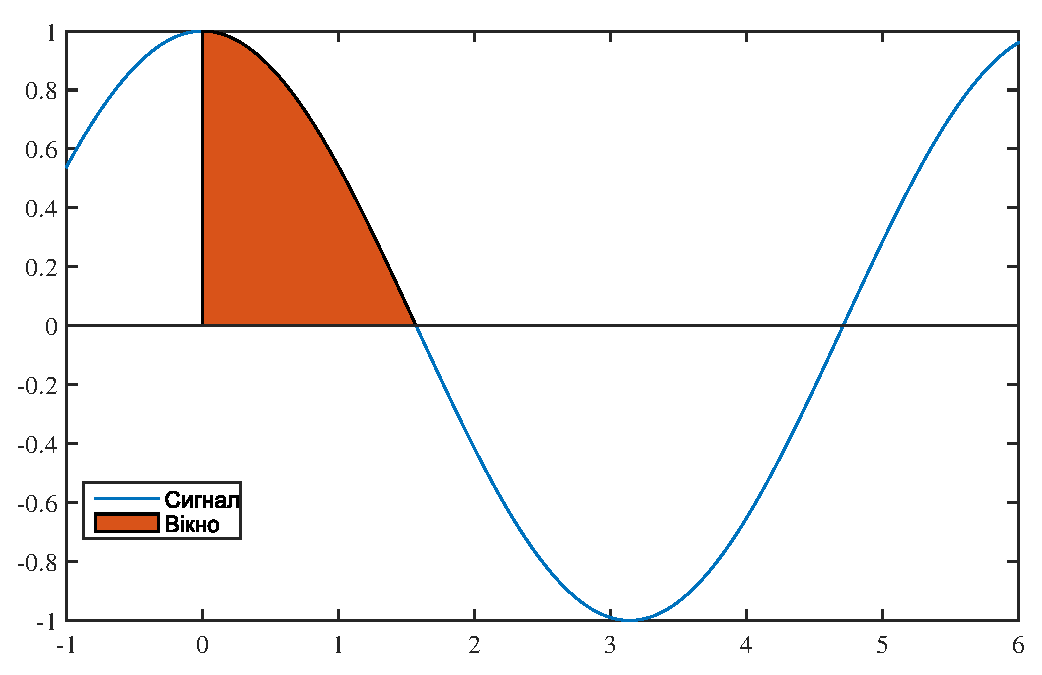
\includegraphics[width=\textwidth]{rect-applicated.eps}
                    \caption{Результат застосування прямокутного вікна}
                    \label{fig:rekt-appl}
                \end{figure}
            \item Вікно Гана (Hann window).
                Ця функція названа на честь Жуліуса фон Гана (Julius von Hann) й має наступний аналітичний запис:
                \begin{equation}
                    w( n ) = \frac12 \left( 1 - \cos{ \frac{ 2 \pi n}{N - 1}} \right)
                \end{equation}

                Ця функція приймає нульові значення на кінцях вікна.

                Вигляд вагової функції"=вікна зображено на малюнку~\ref{fig:hanning}, а результат застосування до
                (ко)синусоіди --- на рисунку~\ref{fig:hanning-appl}.

                \stepcounter{figurecount}
                \begin{figure}[h]
                    \centering
                    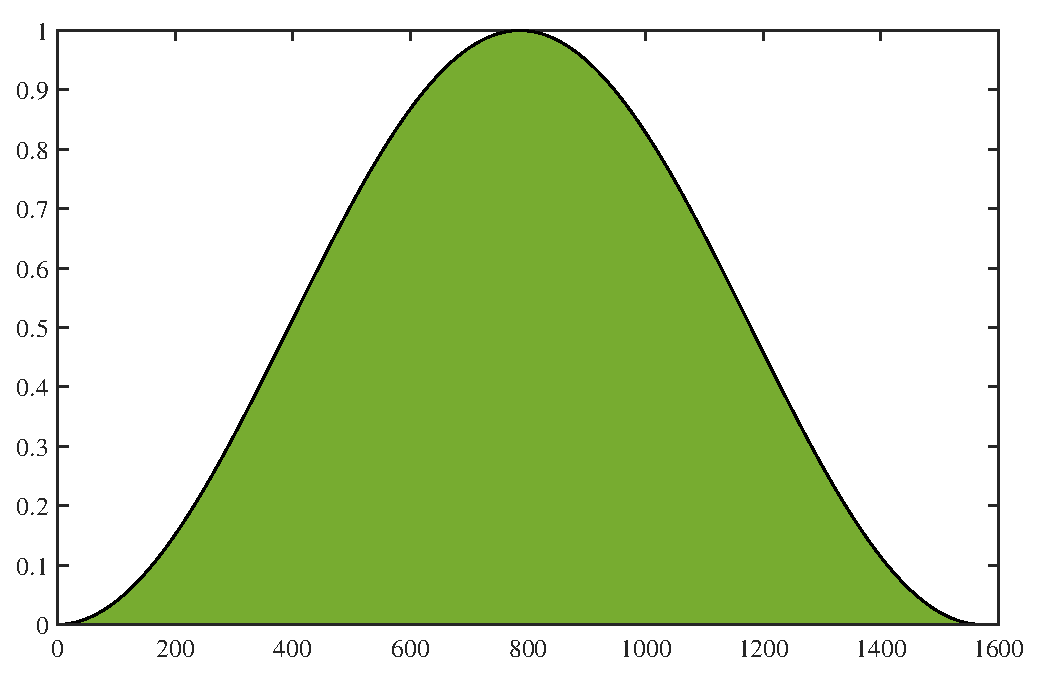
\includegraphics[width=\textwidth]{hanning.eps}
                    \caption{Вигляд вікна Гана}
                    \label{fig:hanning}
                \end{figure}

                \stepcounter{figurecount}
                \begin{figure}[h]
                    \centering
                    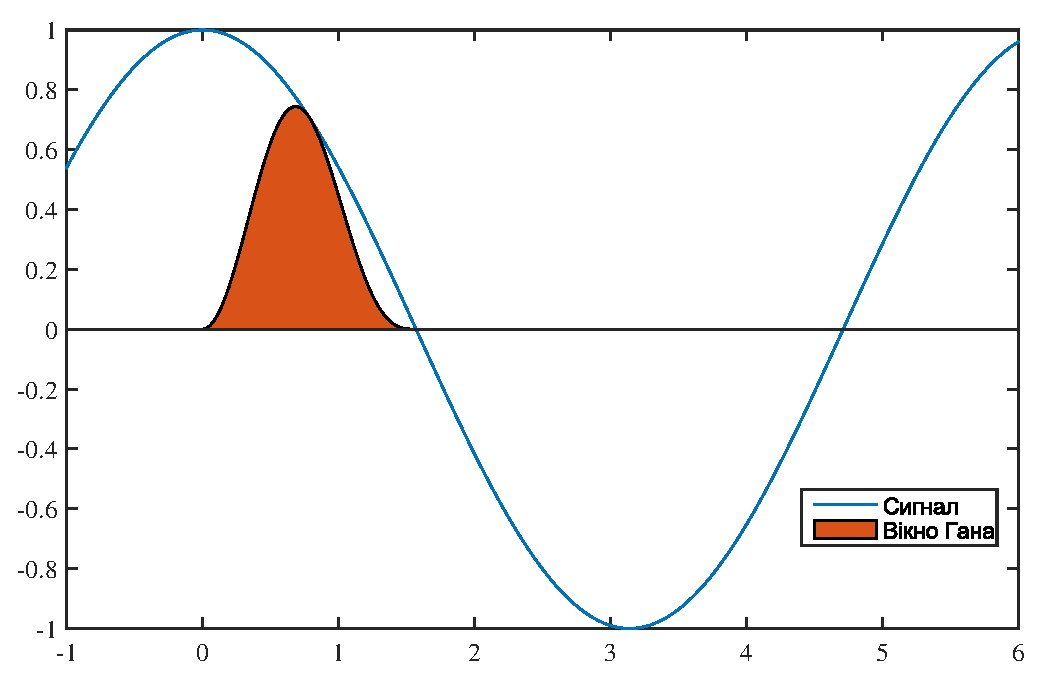
\includegraphics[width=\textwidth]{hanning-appl.eps}
                    \caption{Результат застосування вікна Гана}
                    \label{fig:hanning-appl}
                \end{figure}
            \item Вікно Геммінга.
                Це вікно має наступний аналітичний запис:
                \begin{equation}
                    w(n) = \frac{25}{46} - \frac{21}{46}\cos{ \frac{ 2 \pi n}{N - 1}}
                \end{equation}
                Це вікно значно зменшує рівень бокових пелюсток при перетворенні Фур’є.

                Вигляд вагової функції"=вікна зображено на малюнку~\ref{fig:hamming}, а результат застосування до
                (ко)синусоіди --- на рисунку~\ref{fig:hamming-appl}.

                \stepcounter{figurecount}
                \begin{figure}[h]
                    \centering
                    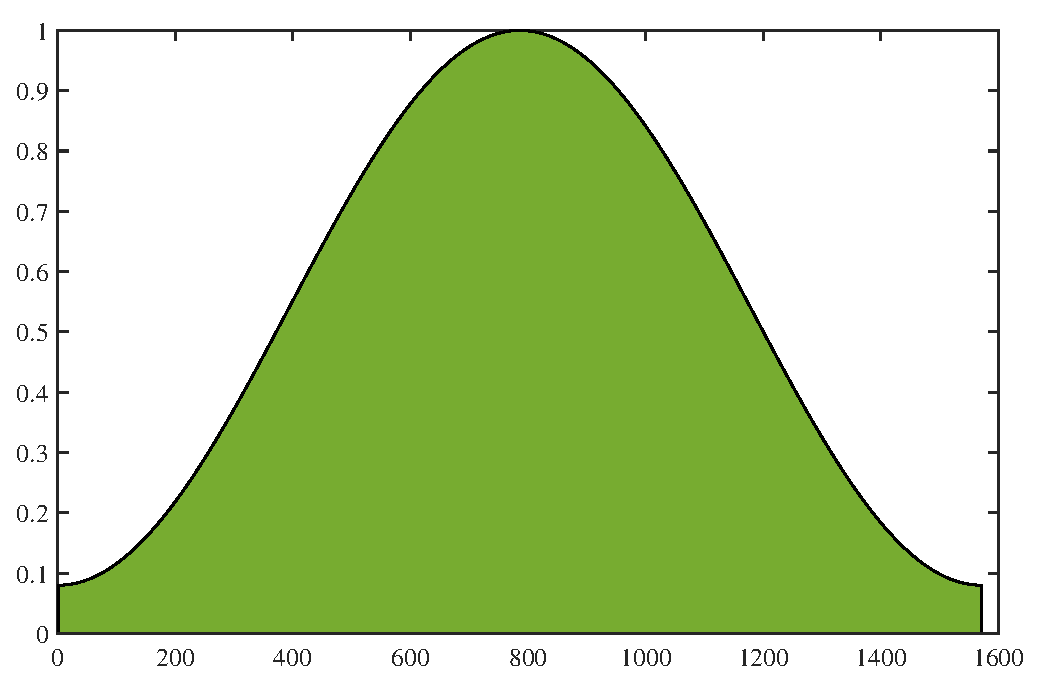
\includegraphics[width=\textwidth]{hamming.eps}
                    \caption{Вигляд вікна Геммінга}
                    \label{fig:hamming}
                \end{figure}

                \stepcounter{figurecount}
                \begin{figure}[h]
                    \centering
                    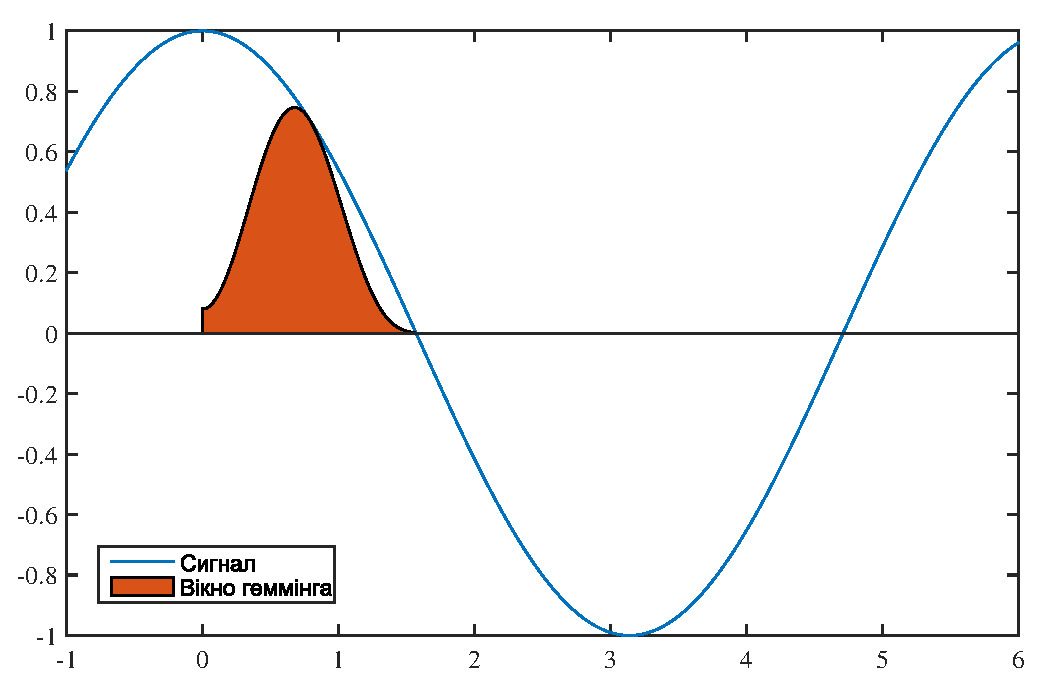
\includegraphics[width=\textwidth]{hamming-appl.eps}
                    \caption{Результат застосування вікна Геммінга}
                    \label{fig:hamming-appl}
                \end{figure}
        \end{enumerate}

\section{Опис існуючих методів}
    \subsection{Взаємокореляція}
        Взаємокореляція (cross-correlation) являє собою міру подібності двох функцій (сигналів), одна з яких
        зсувається відносно іншої.

        Для дискретного сигналу взаємокореляція має вигляд:
        \begin{equation}
            CC(f,g)[ n ] \equiv (f \star g)[ n ] \defeq \frac{1}{k}\sum\limits_{m=1}^{k} f^*[m] g[ m + n ]
        \end{equation}

        Для використання цього методу необхідно взяти в якості сигналу $f$ вхідний сигнал, $g$ --- шаблон, що
        шукається; в якості $k$ необхідно взяти довжину (кількість значень) шаблону $g$.

        Ідея полягає в тому, що сума добутків значень шаблону на вхідний сигнал буде тим більше, чим більше вхідний
        сигнал схожий на шаблон на обраному проміжку.

        Значним недоліком цього методу є залежність від амплітуди сигналу: якщо сигнал має на деякому проміжку
        амплітуду, значно більшу за середню амплітуду сигналу та шаблону, то значення взаємокореляції між сигналом та
        шаблоном на цьому проміжку буде значно більше, ніж значення взаємокореляції між шаблоном та шаблоном
        (автокореляція).

        Саме тому більш практичним вважається використання нормалізованої взаємокореляції.
    \subsection{Нормалізована взаємокореляція}
        Нормалізована взаємокореляція шукається як взаємокореляція між сигналами, що нормалізовані.
        Як правило, під нормалізацією розуміється віднімання від сигналу середнього значення на проміжку й ділення на
        середньо"=квадратичне відхілення на цьому проміжку.

        Для дискретного сигналу нормалізована взаємокореляція має вигляд:
        \begin{align}
            NCC(f,g)[ n ] &\defeq \frac{1}{k} \sum\limits_{m=1}^{k} \tilde{f_n}^*[m] \tilde{g}[ m + n ],\\
            \tilde{f_n}[m] &\defeq \frac{f[m] - \bar{f_n}}{\sigma_{f_n}},\\
            \tilde{g}[m]   &\defeq \frac{g[m] - \bar{g}}{\sigma_g}
        \end{align}
        де $\sigma_{f_n}$ --- середньо"=квадратичне відхілення вікна вхідного сигналу $f$, $\sigma_g$ ---
        середньо"=квадратичне відхилення шаблону $g$, $\bar{f_n}$ --- середнє значення вхідного сигналу на проміжку
        вікна, а $\bar{g}$ --- середнє значення шаблону.

        Цей метод дозволяє знаходити шаблон, навіть якщо вхідний сигнал має значні \invcommas{спалахи} амплітуди.
        Також нормалізація шаблону дозволяє знаходити в сигналі шаблон із зміненої амплітудою.

        Завдяки тому, що значення цієї метрики лежать в межах від ${-1}$ до $1$, задача пошуку порогу $e_0$ значно
        спрощується.

    \subsection{Сума квадратів відстаней}
        Метод полягає в пошуку квадрату відстані між $k$"=вимірного вектору шаблону та обраного вікна сигналу.

        Для дискретного сигналу це буде наступна залежність:
        \begin{equation}
            \text{SSD}\left(f, g\right)[ n ] \defeq \frac{1}{k}\sum\limits_{m=1}^k {\left(f[m] - g[m]\right)}^2
        \end{equation}

        Отримана функціональна залежність характеризує відстань кожного вікна вхідного сигналу до шаблону.
        Таким чином, чим менше ця відстань --- тим більше сигнал у обраному вікні схожий до шаблону.

        На відміну від методу взаємокореляцій, на ефективність методу пошуку суму квадратів відстаней не впливає
        значення амплітуди сигналу.
    \subsection{Нормалізована сума квадратів відстаней}
        Аналогічно до нормалізованої взаємокореляції можна визначити нормалізовану суму квадратів відстаней:
        \begin{equation}
            \text{NSSD}\left(f, g\right)[ n ] \defeq \frac{1}{k}\sum\limits_{m=1}^k {\left(\tilde{f}[m] - \tilde{g}[m]\right)}^2
        \end{equation}

\section{Порівняльний аналіз методів}
\label{s:existing-compare}
    В таблиці~\ref{tab:existing} підсумовані основні характеристики розглянутих методів.
    Слід зазначити, що підрахування взаємокореляції можна значно прискорити завдяки (швидкому) перетворенню Фур’є
    (FFT).

    \stepcounter{tablecount}
    \begin{table}{|p{0.1\textwidth}|p{0.2\textwidth}|p{0.3\textwidth}|p{0.29\textwidth}|}
        {Порівняння існуючих методів}{tab:existing}
        {\hline
            & Складність обчислень & Стійкість до зміни амплітуди шаблону & Стійкість до артефактів вхідного сигналу\\
        \hline}

        CC   & $O(k n)$   & $-$ & $-$\\
        NCC  & $O(2 k n)$ & $+$ & $+$\\
        SSD  & $O(k n)$   & $-$ & $+$\\
        NSSD & $O(2 k n)$ & $+$ & $+$\\
    \end{table}

    Як можна побачити, найпоширеніші методи, що застосовуються для сигналів загального виду, є дуже чутливими до
    зміни шаблону: тільки метод нормалізованої взаємокореляції дозволяє коректно знаходити шаблон із лінійно"=зміненою
    амплітудою.
%TODO Вставити посилання
    Експерименти показали, що ці методи не знаходять шаблон в сигналі, якщо амплітуда шаблону змінювалася не сталим
    чином.

\section{Висновки}
Було розглянуто предметну область поставленої задачі, описані такі методи, як метод ковзного вікна та віконні функції.
Також було розглянуто найпоширеніші існуючі методи пошуку шаблонів й порівняно їх характеристики.

За результатом цього порівняння було визначено, що розглянуті методи при досить гарній швидкодії знаходять такі
шаблони, що були змінені майже пропорційно.
Тобто шаблони, що деформують з різною силою будуть погано знаходитись цими методами.

Саме тому в наступному розділі буде запропоновано використання розкладення функції в поліноми Кунченка як метод пошуку
шаблонів.

% vim: spelllang=uk,en spell filetype=tex
